
\begin{figure}
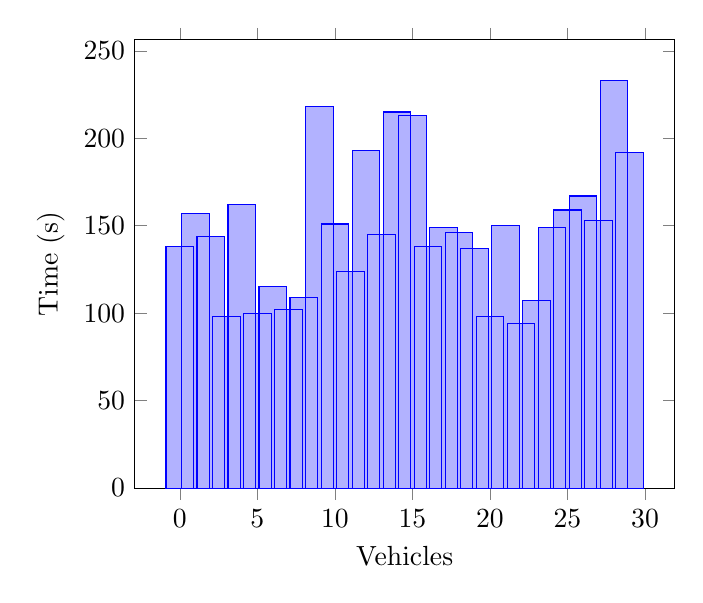
\begin{tikzpicture}
\begin{axis}[
legend style={anchor=west},
xlabel=Vehicles,
ylabel=Time (s),
ymin=0,
ybar,
]
\addplot coordinates {
(0, 138)
(1, 157)
(2, 144)
(3, 98)
(4, 162)
(5, 100)
(6, 115)
(7, 102)
(8, 109)
(9, 218)
(10, 151)
(11, 124)
(12, 193)
(13, 145)
(14, 215)
(15, 213)
(16, 138)
(17, 149)
(18, 146)
(19, 137)
(20, 98)
(21, 150)
(22, 94)
(23, 107)
(24, 149)
(25, 159)
(26, 167)
(27, 153)
(28, 233)
(29, 192)
};

\end{axis}
\end{tikzpicture}
\label{tik:100:21_V, 20_V, 17_N, 15_S, 15_S.-30, 13_N, 13_N.-40, 11_N, 8_N, 7_N, 7_N.-60, 5_N, 4_N, 4_N.-60, 1_N}
\caption{100 percent diving with GSC on route $21_V, 20_V, 17_N, 15_S, 15_S.-30, 13_N, 13_N.-40, 11_N, 8_N, 7_N, 7_N.-60, 5_N, 4_N, 4_N.-60, 1_N$}
\end{figure}
